\section{Example: Odds Ratio in Paired and Unpaired Data}
Suppose we have the following data.
\begin{figure}[H]
	\centering
	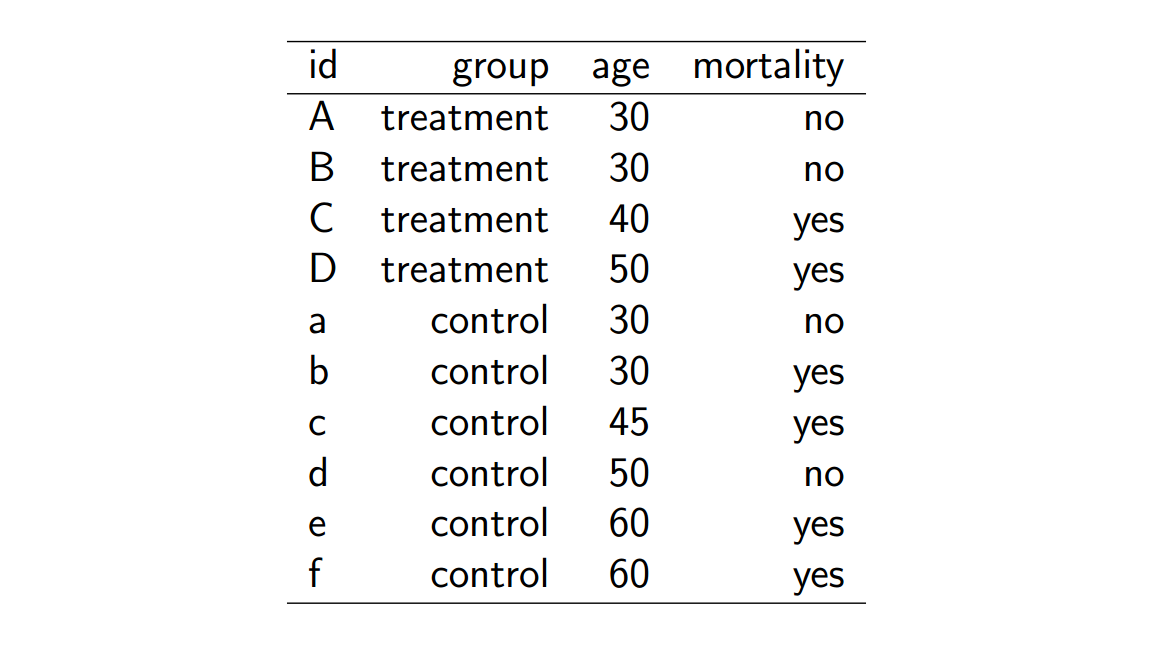
\includegraphics[width=0.7\linewidth]{fig/screenshot001}
	\caption{Example Data}
	\label{fig:screenshot001}
\end{figure}

\subsection{Review: $2 \times 2$ Contingency Table}
The data can be represented by the following contingency table.
\begin{figure}[H]
	\centering
	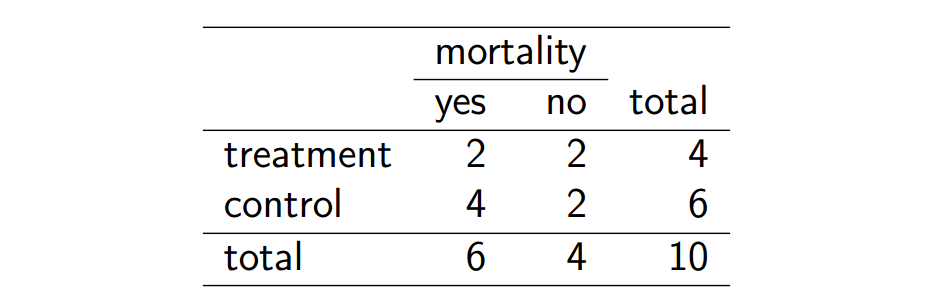
\includegraphics[width=0.7\linewidth]{fig/screenshot002}
	\caption{Contingency Table}
	\label{fig:screenshot002}
\end{figure}

The odds ratio is the ratio of two odds
\[
\theta 
= 
\frac
{\frac{\P(\text{Yes}|\text{Treatment})}{\P(\text{No}|\text{Treatment})}}
{\frac{\P(\text{Yes}|\text{Treatment})}{\P(\text{No}|\text{Treatment})}}
=\frac{\P(\text{Yes}|\text{Treatment})\P(\text{No}|\text{Treatment})}
{\P(\text{No}|\text{Treatment})\P(\text{Yes}|\text{Treatment})}
\]

In the sample,
\begin{itemize}
	\item Proportion of mortality in the treatment group: $2/4 = 0.5$.
	\item Proportion of mortality in the control group: $4/6 = 0.67$.
	\item The estimated odds in the treatment group: $2/2 = 1$.
	\item The estimated odds in the control group: $4/2 = 2$.
\end{itemize}

Therefore, the estimated odds ratio is
\[\hat{\theta} = \frac{2 \times 2}{4 \times 2} = \frac{1}{2}\]

\subsection{Matching for Paired Data}
To eliminate the effect of age for mortality, we can pair the data as follows, where treatment id and matched id are matched by age.
\begin{figure}[H]
	\centering
	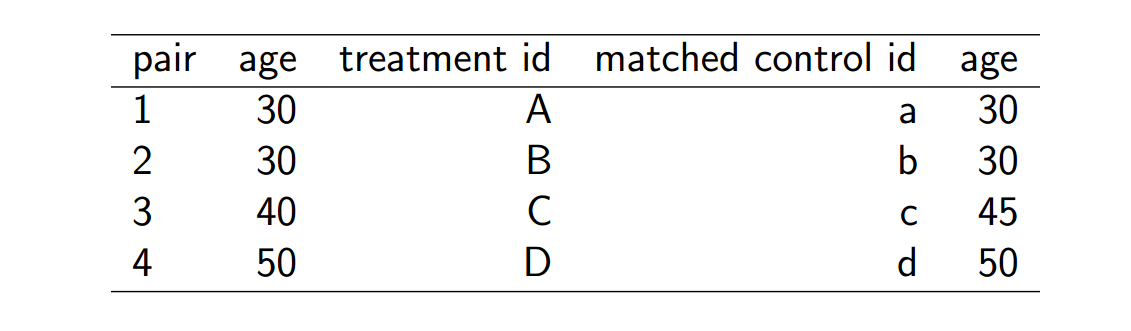
\includegraphics[width=0.7\linewidth]{fig/screenshot003}
	\caption{Matching Data}
	\label{fig:screenshot003}
\end{figure}
The mortality of the matched data is as follows.
\begin{figure}[H]
	\centering
	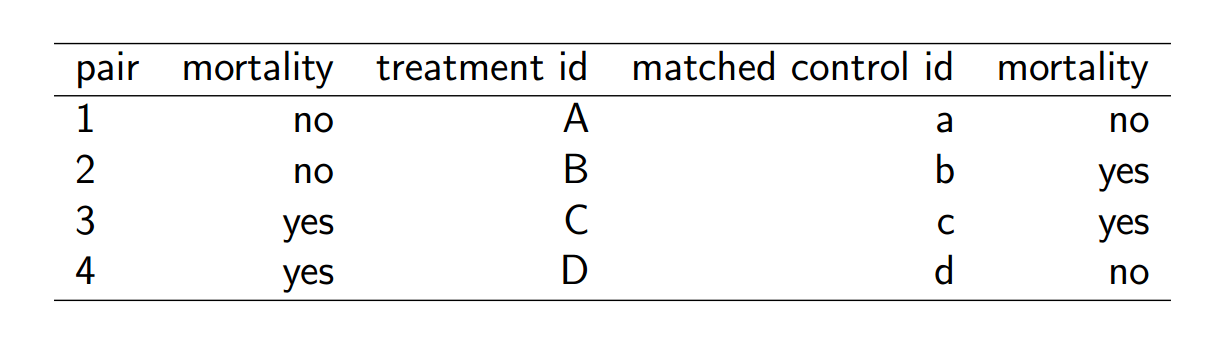
\includegraphics[width=0.7\linewidth]{fig/screenshot004}
	\caption{Mortality of Matched Data}
	\label{fig:screenshot004}
\end{figure}

The frequency of mortality in each group can be represented by the following table.
\begin{figure}[H]
	\centering
	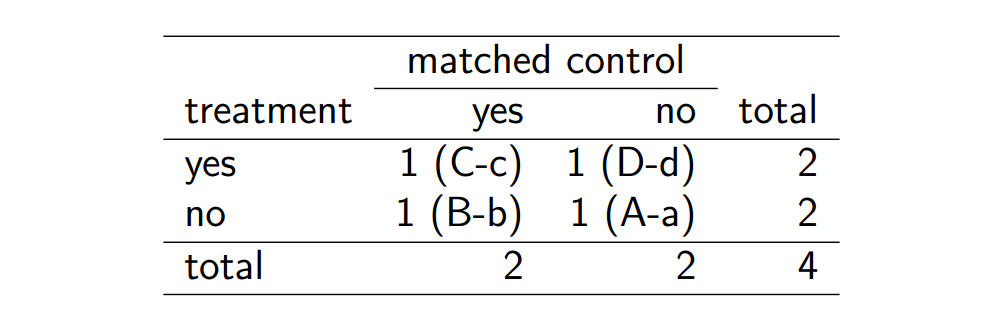
\includegraphics[width=0.7\linewidth]{fig/screenshot005}
	\caption{Contingency Table for Paired Data}
	\label{fig:screenshot005}
\end{figure}

After matching, in the paired sample,
\begin{itemize}
	\item Proportion of mortality in the treatment group: $2/4 = 0.5$. (Sum of first row)
	\item Proportion of mortality in the control group: $2/4 = 0.5$. (Sum of first column)
\end{itemize}

The odds ratio is 
\[\lambda = 
\frac
{\P[(\text{Yes}|\text{Treatment}) \& (\text{No}|\text{Matched Control})]}
{\P[(\text{No}|\text{Treatment}) \& (\text{Yes}|\text{Matched Control})]}
\]

The estimated odds ratio is
\[
\hat{\lambda} = 
\frac{1 (\text{from pair D-d})}{1 (\text{from pair B-b})} = 1
\]
